\begin{frame}
    \frametitle{Outline}
    \begin{enumerate}
		\item Linear splitting trees
			\begin{itemize}
				\item Upper bounds
				\item Lower bounds for Pigeonhole and 2-fold Tseitin formulas
			\end{itemize}

		\item Proof system Res-Lin 
			\begin{itemize}
				\item Semantic and syntactic version are equivalent
				\item Implication completeness
				\item Simulation in R(lin)
			\end{itemize}

	\end{enumerate}
\end{frame}


\begin{frame}
    \frametitle{Splitting trees}
    $(\lnot x \lor y) \land (x \lor \lnot y) \land (\lnot y \lor z) \land
    	(y \lor \lnot z) \land (x \lor z) \land (\lnot x \lor \lnot z)$ 
	\only<1>{\input{pics/DPLL_tree_new.tex}}
	\only<2>{\tikzstyle{end} = [circle, minimum size = 0.1cm, draw, inner sep = 0.1pt]
\tikzstyle{leaf} = [circle, minimum size = 0.6cm, draw, inner sep = 0.1pt, blue]
            
\tikzstyle{level 1}=[level distance = 1.5cm, sibling distance = 5cm]
\tikzstyle{level 2}=[sibling distance = 4cm]
\tikzstyle{level 3}=[sibling distance = 1.5cm]
    
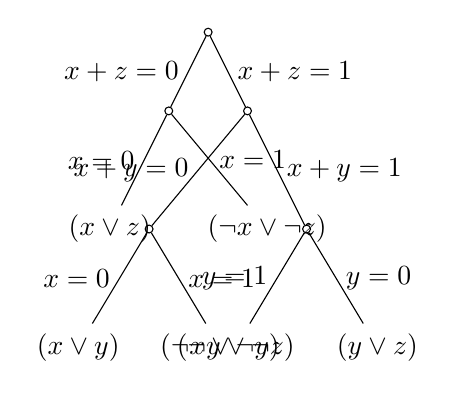
\begin{tikzpicture}[label distance=8mm]
	\node [end] {}
        child {
        	node[end] {}
           	child {
               	node {\alert{$(x \lor z)$}}
                edge from parent
	            node[left] {$x = 0$}
            }
            child[sibling distance = 2.5cm] {
               	node {\alert{$(\neg x \lor \neg z)$}}
                edge from parent
	            node[right] {$x = 1$}
            }
           	edge from parent
            node[left] {$x + z = 0$}
        }
        child {
        	node[end] {}
            child[sibling distance = 2.5cm] {
                node[end] {}
                child {
            		node {\alert{$(x \lor y)$}}
	                edge from parent
    	            node[left] {$x = 0$}
        	    }
                child {
            		node {\alert{$(\neg x  \lor \neg y)$}}
                	edge from parent
	                node[right] {$x = 1$}
    	        }
                edge from parent
                node[left] {$x + y = 0$}
            }
            child {
            	node[end] {}
                child {
            		node {\alert{$(\neg y \lor \neg z)$}}
	                edge from parent
    	            node[left] {$y = 1$}
        	    }
                child {
            		node {\alert{$(y \lor z)$}}
                	edge from parent
	                node[right] {$y = 0$}
    	        }
                edge from parent
                node[right] {$x + y = 1$}
            }
           	edge from parent
            node[right] {$x + z = 1$}
        };
\end{tikzpicture}

%%% Local Variables: 
%%% mode: latex
%%% TeX-master: t
%%% End: 
}
\end{frame}



\begin{frame}
    \frametitle{Linear splitting trees (LST)}
	Solving CNF SAT using splitting by linear forms over $\mathbb{F}_2$
    \begin{columns}
        \begin{column}{3cm}
            Degenerate leaf
            \tikzstyle{end} = [circle, minimum size = 0.1cm, draw, inner sep = 0.1pt]
\tikzstyle{leaf} = [circle, minimum size = 0.6cm, draw, inner sep = 0.1pt, blue]
            
\tikzstyle{level 1}=[level distance = 1cm, sibling distance = 1.5cm]
\tikzstyle{level 2}=[level distance = 1.5cm, sibling distance = 2cm]
\tikzstyle{level 3}=[level distance = 1.5cm, sibling distance = 2cm]


    
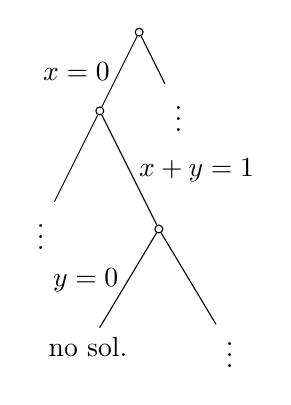
\begin{tikzpicture}[label distance = 8mm]
	\node [end] (z){}
        child {
        	node[end] (b) {}
            child {
    			node {$\vdots$}
		        edge from parent
	    		node[left] {}
			}
		    child {
		        node[end] {}
                child {
                  	node {\alert{no sol.}}
                    edge from parent
                    node[left] {$y = 0$}
                }
                child {
        			node {$\vdots$}
		           	edge from parent
        		    node[right] {}
		        }
	            edge from parent
		        node[right] {$x + y = 1$}
            }
           	edge from parent
            node[left] {$x = 0$}
        }
        child {
        	node (b) {$\vdots$}
           	edge from parent
            node[right] {}
        };
\end{tikzpicture}

%%% Local Variables: 
%%% mode: latex
%%% TeX-master: t
%%% End: 

        \end{column}
        \begin{column}{3cm}
            Sat. assignment
            \tikzstyle{end} = [circle, minimum size = 0.1cm, draw, inner sep = 0.1pt]
\tikzstyle{leaf} = [circle, minimum size = 0.6cm, draw, inner sep = 0.1pt, blue]
            
\tikzstyle{level 1}=[level distance = 1cm, sibling distance = 1cm]
\tikzstyle{level 2}=[level distance = 1.5cm, sibling distance = 1.5cm]
\tikzstyle{level 3}=[level distance = 1.5cm, sibling distance = 1.8cm]


    
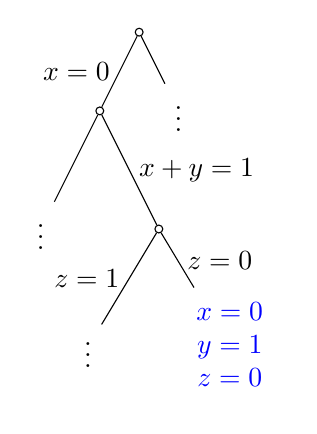
\begin{tikzpicture}[label distance = 8mm]
	\node [end] (z){}
        child {
        	node[end] (b) {}
            child {
    			node {$\vdots$}
		        edge from parent
	    		node[left] {}
			}
		    child {
		        node[end] {}
                child {
        			node {$\vdots$}
		           	edge from parent
        		    node[left] {$z = 1$}
		        }
                child {
                  	node[blue] {\begin{tabular}{c} $x = 0$ \\ $y = 1$ \\ $z = 0$ \end{tabular}}
                    edge from parent
                    node[right] {$z = 0$}
                }
	            edge from parent
		        node[right] {$x + y = 1$}
            }
           	edge from parent
            node[left] {$x = 0$}
        }
        child {
        	node (b) {$\vdots$}
           	edge from parent
            node[right] {}
        };
\end{tikzpicture}

%%% Local Variables: 
%%% mode: latex
%%% TeX-master: t
%%% End: 

        \end{column}
        \begin{column}{3cm}
            Contradiction with a clause
            \input{pics/case_contradiction.tex}
        \end{column}
    \end{columns}
    
	$\Phi$ refutes $(x_1 \lor x_2 \dots \lor x_k)$ iff $\Phi \land (x_i = 1)$ is
    unsatisfiable $\forall i$.
\end{frame}



\begin{frame}
    \frametitle{Algorithm by Seto and Tamaki}

	\begin{itemize}
		\item{} [Seto, Tamaki, 2011] Algorithm for Formula-SAT over the full binary
		    basis. For formulas of size $cn$ the algorithm runs $2^{(1 - \mu_c)n}$,
            where $\mu_c$ is a constant.
		\pitem Splitting over linear combinations.
	\end{itemize}    
\end{frame}


\myframe{Upper bounds}
{
\begin{itemize}
\item Linear systems over $\mathbb{F}_2$
\begin{itemize}
\item Hard for resolution and DPLL
\item Easy for Linear splitting trees
\end{itemize}
\pitem Perfect matching principle for graphs with odd vertices
\begin{itemize}
\item Hard for resolution and DPLL [Razborov, 2003]
\item Easy for Linear splitting trees
\end{itemize}
\pitem Pebbling contradictions
\begin{itemize}
\item
For CNF $\phi$ we denote by $\phi^{\oplus}$ a CNF formula
obtained from $\phi$ by substituting $x_1\oplus x_2$ for each variable $x$. 
\item{} [Urquhart,2011] The size of tree-like Resolution of $\phi^{\oplus}$ is at least $2^{d(\phi)}$, where $d(\phi)$ is 
the minimal depth of the resolution proof of $\phi$. 
\item{} [Urquhart,2011] Pebbling contradictions $Peb(G_n)$ such that $d(Peb(G_n))=\Omega(n/\log n)$ 
and $Peb(G_n)$ has $O(n)$ tree-like resolution proof. 
\item Tree-like resolution proof of $Peb^\oplus(G_n)$ is at least $2^{n/\log n}$, while $Peb^\oplus(G_n)$ has $O(n)$-size LST.
\end{itemize}
\end{itemize}


%\begin{tabular}{|c|c|c|c|}
%\hline
%Formulas & Resolution & Tree-like & LST \\
%&& Resolution(DPLL)&\\
%\hline
%Linear systems & $2^{\Omega(n)}$ & $2^{\Omega(n)}$& poly(n)\\
%(Tseitin formulas)&&&\\
%\hline
%Perfect Matching & $2^{\Omega(n)}$ & $2^{\Omega(n)}$& poly(n)\\
%Principle for graph&&&\\
%with odd vertices&&&\\
%\hline
%Peb($G_n$) & $poly(n)$ & $poly(n)$& $poly(n)$\\
%\hline
%Peb$^\oplus(G_n)$ & $poly(n)$ & $2^{n/log n}$& $poly(n)$\\
%\hline

%Linear systems & $2^{\Omega(n)}$ & $2^{\Omega(n)}$& poly(n)\\
%(Tseitin formulas)&&&\\
%\end{tabular}

%What formulas have 
}

\myframe{Linear systems}
{
\begin{columns}
\begin{column}{1cm}
Unsatisfiable system:

$\left\{ \begin{aligned}
f_1=\alpha_1 \\
f_2=\alpha_2 \\
\dots\\
f_m=\alpha_m
\end{aligned}\right.$


\end{column}


\begin{column}{9cm}
\tikzstyle{end} = [thin, circle, minimum size = 0.1cm, draw, inner sep = 0.1pt]
\tikzstyle{leaf} = [thin, circle, minimum size = 0.6cm, draw, inner sep = 0.1pt, blue]
            
\tikzstyle{level 1}=[level distance = 1.5cm, sibling distance = 1.5cm]
\tikzstyle{level 2}=[level distance = 1.5cm, sibling distance = 4cm]
\tikzstyle{level 3}=[level distance = 2cm, sibling distance = 1.5cm]
\tikzstyle{level 4}=[level distance = 2cm, sibling distance = 1.3cm]

\tikzstyle{edge from parent} = [thin, draw]

    
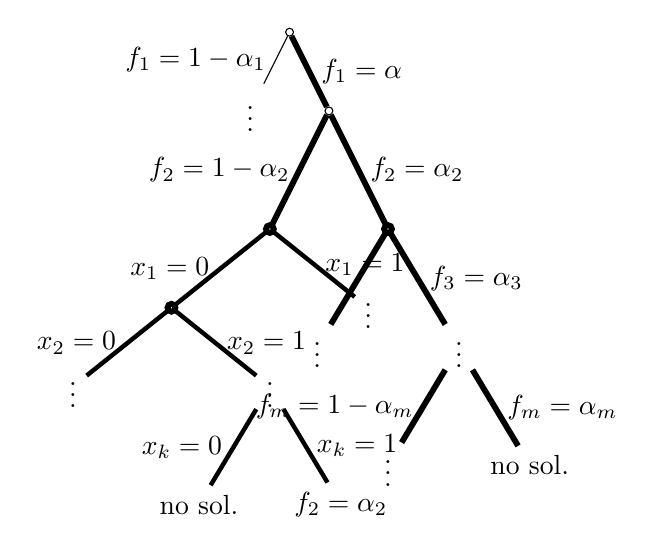
\begin{tikzpicture}[label distance = 8mm]
	\node [end] {}
	    child {
        	node {$\vdots$}
           	edge from parent
            node[left] {$f_1 = 1 - \alpha_1$}
        }
        child {
        	node[end] {}
            child {
		        node[end] {}
                child[level distance = 1.cm, sibling distance = 2.5cm] {
        			node[end] {}
                    child[level distance = 1cm] {
                    	node {$\vdots$}
                    	edge from parent[ultra thick]
	        		    node[left] {$x_2 = 0$}
                    }
                    child[level distance = 1cm] {
                    	node {$\vdots$}
                        child[level distance = 1.5cm, sibling distance = 1.8cm] {
                        	node {\alert{no sol.}}
                            edge from parent[ultra thick]
		        		    node[left] {$x_k = 0$}
                        }
                        child[level distance = 1.5cm, sibling distance = 1.8cm] {
                        	node {\alert{$f_2 = \alpha_2$}}
                            edge from parent[ultra thick]
		        		    node[right] {$x_k = 1$}
                        }
                    	edge from parent[ultra thick]
	        		    node[right] {$x_2 = 1$}
                    }
		           	edge from parent[ultra thick]
        		    node[left] {$x_1 = 0$}
		        }
                child[level distance = 1.cm, sibling distance = 2.5cm] {
                  	node {$\vdots$}
                    edge from parent[ultra thick]
                    node[right] {$x_1 = 1$}
                }
	            edge from parent
		        node[left] {$f_2 = 1 - \alpha_2$}
			}
		    child {
		        node[end] {}
                child {
        			node {$\vdots$}
		           	edge from parent
        		    node[left] {}
		        }
                child {
                  	node {$\vdots$}
                    child{
  		                node {$\vdots$}
			           	edge from parent
        			    node[left] {$f_m = 1 - \alpha_m$}
                    }
                    child{
  		                node {\alert{no sol.}}
			           	edge from parent[line width = 2.1pt]
        			    node[right] {$f_m = \alpha_m$}
                    }
                    edge from parent[line width = 2.1pt]
                    node[right] {$f_3 = \alpha_3$}
                }
	            edge from parent[line width = 2.1pt]
		        node[right] {$f_2 = \alpha_2$}
            }
           	edge from parent[line width = 2.1pt]
            node[right] {$f_1 = \alpha$}
        };
\end{tikzpicture}

%%% Local Variables: 
%%% mode: latex
%%% TeX-master: t
%%% End: 

\end{column}
\end{columns}

$f_2=x_1+\dots+x_k$
}

\myframe{Lower bound for PHP}
{
\begin{itemize}
\item $PHP^m_n$, $m$ pigeons, $n$ holes. 
\item variables $p_{i, j}$, $i \in [m]$, $j \in [n]$; 
$p_{i, j}$: $i$-th pigeon is in the $j$-th hole.
\item Clauses: 
\begin{itemize}
\item \mycolor{blue}{Long} clauses: 
$p_{i, 1} \lor p_{i, 2} \dots \lor p_{i, n}$ for all $i \in [m]$
\item \mycolor{blue}{Short} clauses: $\lnot p_{i, k} \lor \lnot p_{j, k}$ for all $i \neq j
\in [m]$ and all $k \in [n]$.
\end{itemize}
\item $PHP^m_n$ is unsatisfiable iff $m>n$.

\end{itemize}
\pause \myth The size of any LST of $PHP^m_n$ is at least $2^{\frac{n-1}{2}}$.
}

\myframe{Lower bound for PHP}
{
\myth The size of any LST of $PHP^m_n$ is at least $2^{\frac{n-1}{2}}$.

\dok
\begin{columns}
\begin{column}{8.5cm}
\begin{itemize}
\item $\pi$ is \mycolor{blue}{acceptable} if it satisfies all short clauses.
\pitem Consider LST $T$ and cut off all vertices without acceptable solutions. Resulting tree $T'\neq \emptyset$.
%\pitem $T'\neq \emptyset$
\pitem Every leaf in $T'$ refutes some long clause.
\pitem Consider a path $\ell$ in $T'$ from root to leaf. We claim that $\ell$ contains at least $\frac{n-1}{2}$ splitting 
points.
\pitem $\Phi_\ell$ is a set of equations followed by splitting points along $\ell$. $\Phi_\ell$ has no acceptable solutions that sutisfies some long clause.
\end{itemize}
\end{column}
\begin{column}{2cm}
\scalebox{0.6}{\includegraphics{php.jpg}}
\end{column}
\end{columns}
\pause \mylem Let a linear system $Ap = b$ from variables
    $p = (p_{i, j})_{i \in [m], j \in [n]}$ have  $k\le \frac{n-1}{2}$
    equations and have an acceptable solution. Then  $\forall i\in [m] \exists \sigma:$ 
    $\sigma$ is an acceptable solution and satisfies $p_{i, 1} \lor
    p_{i, 2} \lor \dots \lor p_{i,n}$.
}

\myframe{Proof of the Lemma}
{
\mylem Let a linear system $Ap = b$ from variables
    $p = (p_{i, j})_{i \in [m], j \in [n]}$ have $k\le \frac{n-1}{2}$
    equations and have an acceptable solution. Then  $\forall i\in [m] \exists \sigma:$ 
    $\sigma$ is an acceptable solution and satisfies $p_{i, 1} \lor
    p_{i, 2} \lor \dots \lor p_{i,n}$.

\begin{itemize}
\pitem $1\to 0$ can't violate the acceptability.
\pitem Let $\pi$ be acceptable solution with the minimal number of 1's. 
\pitem $\pi$ contains at most $k$ ones.
\begin{itemize}
\pitem Variables with value $1$ in $\pi$: $p_{j_1}, p_{j_2}, \dots, p_{j_{k + 1}}$
\item $\exists \tau\neq 0: A\tau=0$ and support of $\tau$ is in $p_{j_1}, p_{j_2}, \dots, p_{j_{k + 1}}$.
\item $A(\pi+\tau)=b$, $\pi+\tau$ is acceptable.
\end{itemize}
\pitem $\pi$ has $k + 1$ empty holes with numbers $\ell_1, \ell_2, \dots, \ell_{k + 1}$
\pitem $\exists \tau\neq 0: A\tau=0$ and support of $\tau$ is in $p_{i,\ell_1}, p_{i,\ell_2}, \dots, p_{i,\ell_{k + 1}}$.
\item $A(\pi+\tau)=b$, $\pi+\tau$ is acceptable and satisfies $p_{i, 1} \lor p_{i, 2} \lor \dots \lor p_{i,n}$.
\end{itemize}
}

\myframe{Lower bound for 2-fold Tseitin formulas}
{
\begin{itemize}
\item For unsatisfiable $\phi$ a search problem $Search_\phi$: find a
falsified clause given a variable assignment. 
\item We prove that it is possible to transform a splitting tree $T$ into a randomized
communication protocol for the problem $Search_\phi$ of depth $O(\log |T|\log\log|T|)$ if some variables are known by Alice and
other variables are known by Bob. 
\item Use a lower bound on the randomized communication complexity of 
the problem $Search_{TS^2_{G,c}}$ for a 2-fold Tseitin formula $TS^2_{G,c}$ that follows from %\cite{KalSch92} and \cite{BPPT07}.
[Kalyanasundaram, Schintger 1992] and
[Beame, Pitassi, Segerlind, 2007].
\end{itemize}
\pause
\myth In time polynomial in $n$ one may construct a graph $G(V, E)$ on $n$ vertices
    with maximal degree bounded by a constant and a function $c: V\to \mathbb{F}_2$
    such that the size of any linear splitting tree of $TS^2_{(G,c)}$ is at least
    $\Omega\left(2^{n^{1/3} / \log^3(n)}\right)$.
}

\myframe{Res-Lin}
{
\begin{itemize}
\item Literal: $L=x_{1}+x_{2}+\dots + x_{k}=\alpha$, $\lnot L=x_{1}+x_{2}+\dots + x_{k}=\alpha+1$
\item Linear clause: $\bigvee_i x_{i,1}+x_{i_2}+\dots + x_{i, k_i}=\alpha_i$ or $\lnot \bigwedge x_{i,1}+x_{i_2}+\dots + x_{i, k_i}=1+\alpha_i$.
\pitem Res-Lin:
\begin{itemize}
\item Resolution rule: $\frac{(f = 0) \lor D, (f = 1) \lor D'}{D \lor D'}$
\item Weakening rule: $\frac{C}{C'}$ if $C$ semantically implies $C'$
\end{itemize}
\item \mycolor{blue}{Tree-like} Res-Lin is equivalent to LST.
\end{itemize}
\only<2>{\scalebox{0.8}{\includegraphics{resdpll.jpg}}}
}           



\myframe{Res-Lin vs Sem-Lin}
{
\begin{itemize}
\item Sem-Lin
\begin{itemize}
\item Semantic rule: $\frac{C_1, C_2}{C'}$ if $C_1\land C_2$ semantically implies $C'$
\item Weakening rule: $\frac{C}{C'}$ if $C$ semantically implies $C'$
\end{itemize}
\end{itemize}

\pause\myth Res-Lin p-simulates Sem-lin.

\pause\myex How to get $(x + y = 0)$ from $(x = 0)$ and $(y = 0)$ in Res-Lin? 
\begin{itemize}
\item $\frac{(x = 0)}{(x + y = 0) \lor (y = 1)}$
\item $\frac{(x + y = 0) \lor (y = 1),(y = 0)}{(x + y = 0)}$.
\end{itemize}

\pause
\myth Res-Lin is implication complete.

\begin{itemize}
\pitem The weakening rule may be simulated by a polynomial number of pure syntactic rules: 
\begin{itemize}
\item The simplification rule: $\frac{D\lor (0=1)}{D}$; 
\item The syntactic weakening rule:  $\frac{D}{D\lor (f=\alpha)}$; 
\item The addition rule: $\frac{D\lor (f_1=\alpha_1)\lor (f_2=\alpha_2)}{D\lor (f_1=\alpha_1)\lor (f_1+f_2=\alpha_1+\alpha_2+1)}$
\end{itemize}
\end{itemize}
}

%\end{document}

\myframe{R(lin)}
{
\begin{itemize}
\item R(lin) [Raz, Tsameret, 2007] operates with disjunction of linear equalities with \mycolor{blue}{integer} coefficients.
\item Resolution rule: $\frac{A\lor (F_1=a_1), B\lor (F_2=a_2)}{A \lor B \lor (F_1 \pm F_2=a_1\pm a_2)}$ and
\item Weakening rule: $\frac{A}{A\lor (F=a)}$
\item Simplification rule:  $\frac{B\lor (0=c)}{B}$, where $c\neq 0$.
\end{itemize}

\pause \myth R(lin) p-similates Res-Lin.
\medskip

\pause
\begin{columns}
\begin{column}{5cm}
$x_1+x_2+\dots+x_n\equiv 0 \bmod 2$:
$\left[\begin{aligned} x_1+&\dots+x_n=0\\ x_1+&\dots+x_n = 2 \\ &\dots \\ x_1+&\dots+x_n = 2\lceil n/2\rceil \end{aligned}\right.$
\end{column}
\begin{column}{5cm}
$x_1+x_2+\dots+x_n\equiv 1 \bmod 2$:
$\left[\begin{aligned} x_1+&\dots+x_n=1\\ x_1+&\dots+x_n = 3 \\ &\dots \\ x_1+&\dots+x_n = 2\lceil (n-1)/2\rceil+1 \end{aligned}\right.$
%$(x_1+x_2+\dots+x_n=1)\lor (x_1+x_2+\dots+x_n = 3)\lor \dots \lor (x_1+x_2+\dots+x_n = 2\lceil (n-1)/2\rceil+1)$.
\end{column}
\end{columns}

}

\myframe{Futher research}
{
\begin{itemize}
\item Prove lower bound for daglike Res-Lin.
\item What is tree-like Res-Lin complexity of the Perfect Matching Principle for $K_{n-2,n}$?
\item Does tree-like Res-Lin p-simulate dag-like Resolution?
\item Does PCR p-simulate Res-Lin?
\item Prove lower bound for splitting by linear combinations on \mycolor{blue}{satisfiable} formulas.
\end{itemize}
}



\end{document}
